% coding:utf-8

%----------------------------------------
%FOSAPHY, a LaTeX-Code for a summary of modern control theory
%Copyright (C) 2015, Mario Felder & Michi Fallegger

%This program is free software; you can redistribute it and/or
%modify it under the terms of the GNU General Public License
%as published by the Free Software Foundation; either version 2
%of the License, or (at your option) any later version.

%This program is distributed in the hope that it will be useful,
%but WITHOUT ANY WARRANTY; without even the implied warranty of
%MERCHANTABILITY or FITNESS FOR A PARTICULAR PURPOSE.  See the
%GNU General Public License for more details.
%----------------------------------------

\subsection{Beobachtungsnormalform}
\subsubsection{Signalflussblid}
		\begin{center}
			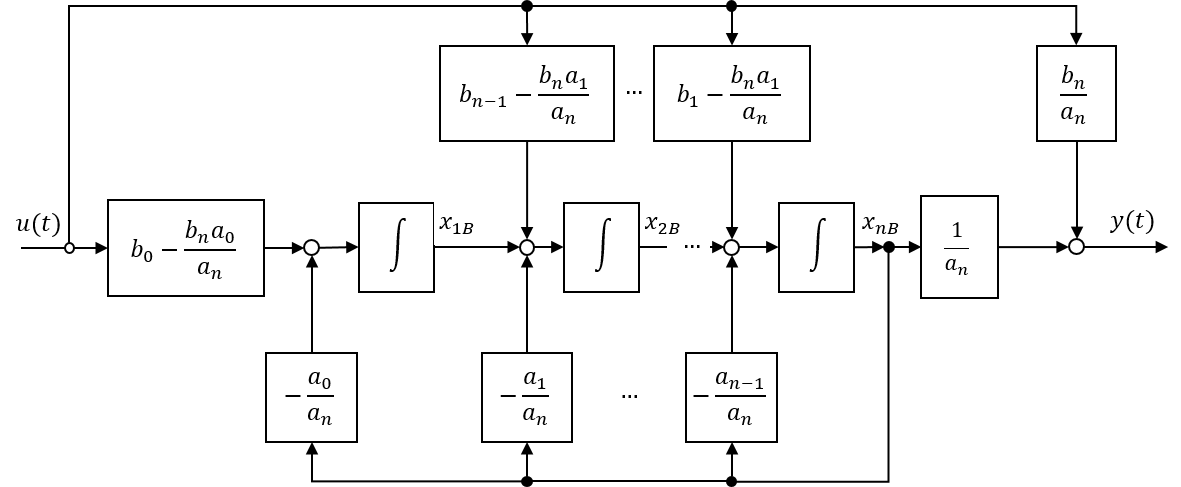
\includegraphics[scale = 0.5]{images/BNF_Signalflussblid.png}
		\end{center}
	\subsubsection{Systemmatrizen}
\[
	\dot x=
	\underbrace{
		\begin{bmatrix}
			0 &	0 & 0 & \ldots & -\frac{a_0}{a_n}\\
			1 & 0 & 0 & \ldots & -\frac{a_1}{a_n}\\
			0 & 1 & 0 & \ldots & -\frac{a_2}{a_n}\\
			\vdots & \vdots & \vdots & \ddots & \vdots \\
			0 & 0 & \ldots & 1 &-\frac{a_{n-1}}{a_n}\\	
		\end{bmatrix}
	}_{\textbf{A}}
	\cdot x +
	\underbrace{
		\begin{bmatrix}
			b_0-b_n\frac{a_0}{a_n} \\
			b_1-b_n\frac{a_1}{a_n} \\
			b_2-b_n\frac{a_2}{a_n}  \\
			\vdots\\
			b_{n-1}-b_n\frac{a_{n-1}}{a_n}\\	
		\end{bmatrix}
	}_{\textbf{b}}
	\cdot u	
\]
\[
	y=
	\underbrace{
			\begin{bmatrix}
				0 & 0 & \ldots & 0 & \frac{1}{a_n}\\
			\end{bmatrix}
	}_{\textbf{$c^T$}}
	\cdot x  +
	\underbrace{
		\left[ \frac{b_n}{a_n} \right] 
	}_{\textbf{d}}
	\cdot u
\]